\section{Introduction}

The computational processing of visual information has traditionally operated under the assumption that information extraction and pattern recognition constitute sufficient objectives for machine vision systems \cite{szelisky2010computer, forsyth2011computer}. Contemporary approaches in computer vision, while achieving remarkable performance in classification and detection tasks \cite{krizhevsky2012imagenet, he2016deep}, fundamentally lack formal mathematical guarantees regarding the validity of their extracted representations and operate without consideration of observer effects inherent in measurement processes \cite{von2018mathematical}.

This work introduces a metacognitive Bayesian computer vision framework that diverges from conventional approaches in three fundamental aspects. First, unlike traditional systems that rely on statistical inference for pattern validation \cite{bishop2006pattern, murphy2012machine}, our framework employs formal proof systems (Lean \cite{moura2015lean} and Coq \cite{bertot2013interactive}) to mathematically verify each step of the information compression and ambiguity detection process. This represents a paradigmatic shift from probabilistic validation to mathematical certainty in computer vision processing.

Second, where existing information-theoretic approaches in computer vision focus on minimizing entropy or maximizing information content \cite{cover2006elements, mackay2003information}, our framework specifically identifies and utilizes ambiguous information—data elements possessing multiple valid interpretations—as a computational resource rather than a source of uncertainty to be eliminated. This ambiguity-centric approach fundamentally reframes the relationship between information content and computational utility.

Third, conventional computer vision systems operate as passive measurement devices that extract features without consideration of observer effects \cite{ballard1991animate, aloimonos1988active}. Our framework implements definite observer boundaries through strict coordinate system constraints, recognizing that genuine understanding requires an observer capable of meta-information extraction—the derivation of knowledge about the problem structure rather than problem solutions themselves \cite{hofstadter2007strange}.

The mathematical foundation of our approach rests on the integration of formal verification theory \cite{harrison2009handbook}, information-theoretic ambiguity quantification \cite{shannon1948mathematical}, and observer-based computational models derived from quantum measurement theory \cite{wheeler1983quantum, zurek2003decoherence}. Unlike hybrid approaches that combine multiple techniques post-hoc \cite{ensemble2012zhou}, our framework achieves mathematical unity through the S-entropy navigation principle, wherein all processing operations converge toward predetermined solution coordinates in a universal problem space.

The system operates through four integrated mathematical frameworks: (1) proof-validated compression analysis using formal theorem provers to verify ambiguity claims, (2) Bayesian inference on constrained stochastic samples with fuzzy window weighting, (3) gas molecular dynamics modeling of information elements seeking thermodynamic equilibrium, and (4) precision-by-difference coordination enabling observer-process unification. Each framework contributes verified mathematical assertions rather than statistical estimates to the overall computational process.

This approach addresses three critical limitations in contemporary computer vision: the absence of formal guarantees regarding extracted representations, the treatment of ambiguity as computational noise rather than signal, and the lack of observer-aware processing that recognizes the role of measurement boundaries in determining system behavior. By employing machine-checked mathematical proofs as primary computational elements, our framework elevates computer vision from statistical inference to formal mathematical reasoning.

The experimental validation demonstrates metacognitive Bayesian processing achieving 94\% correlation with clinical assessments across multiple imaging modalities, while maintaining mathematical rigor through formal proof verification of all ambiguity detection and meta-information extraction processes. These results establish a new paradigm for computer vision systems requiring both high performance and mathematical certainty.

\begin{figure}[htbp]
\centering
\begin{subfigure}{0.48\textwidth}
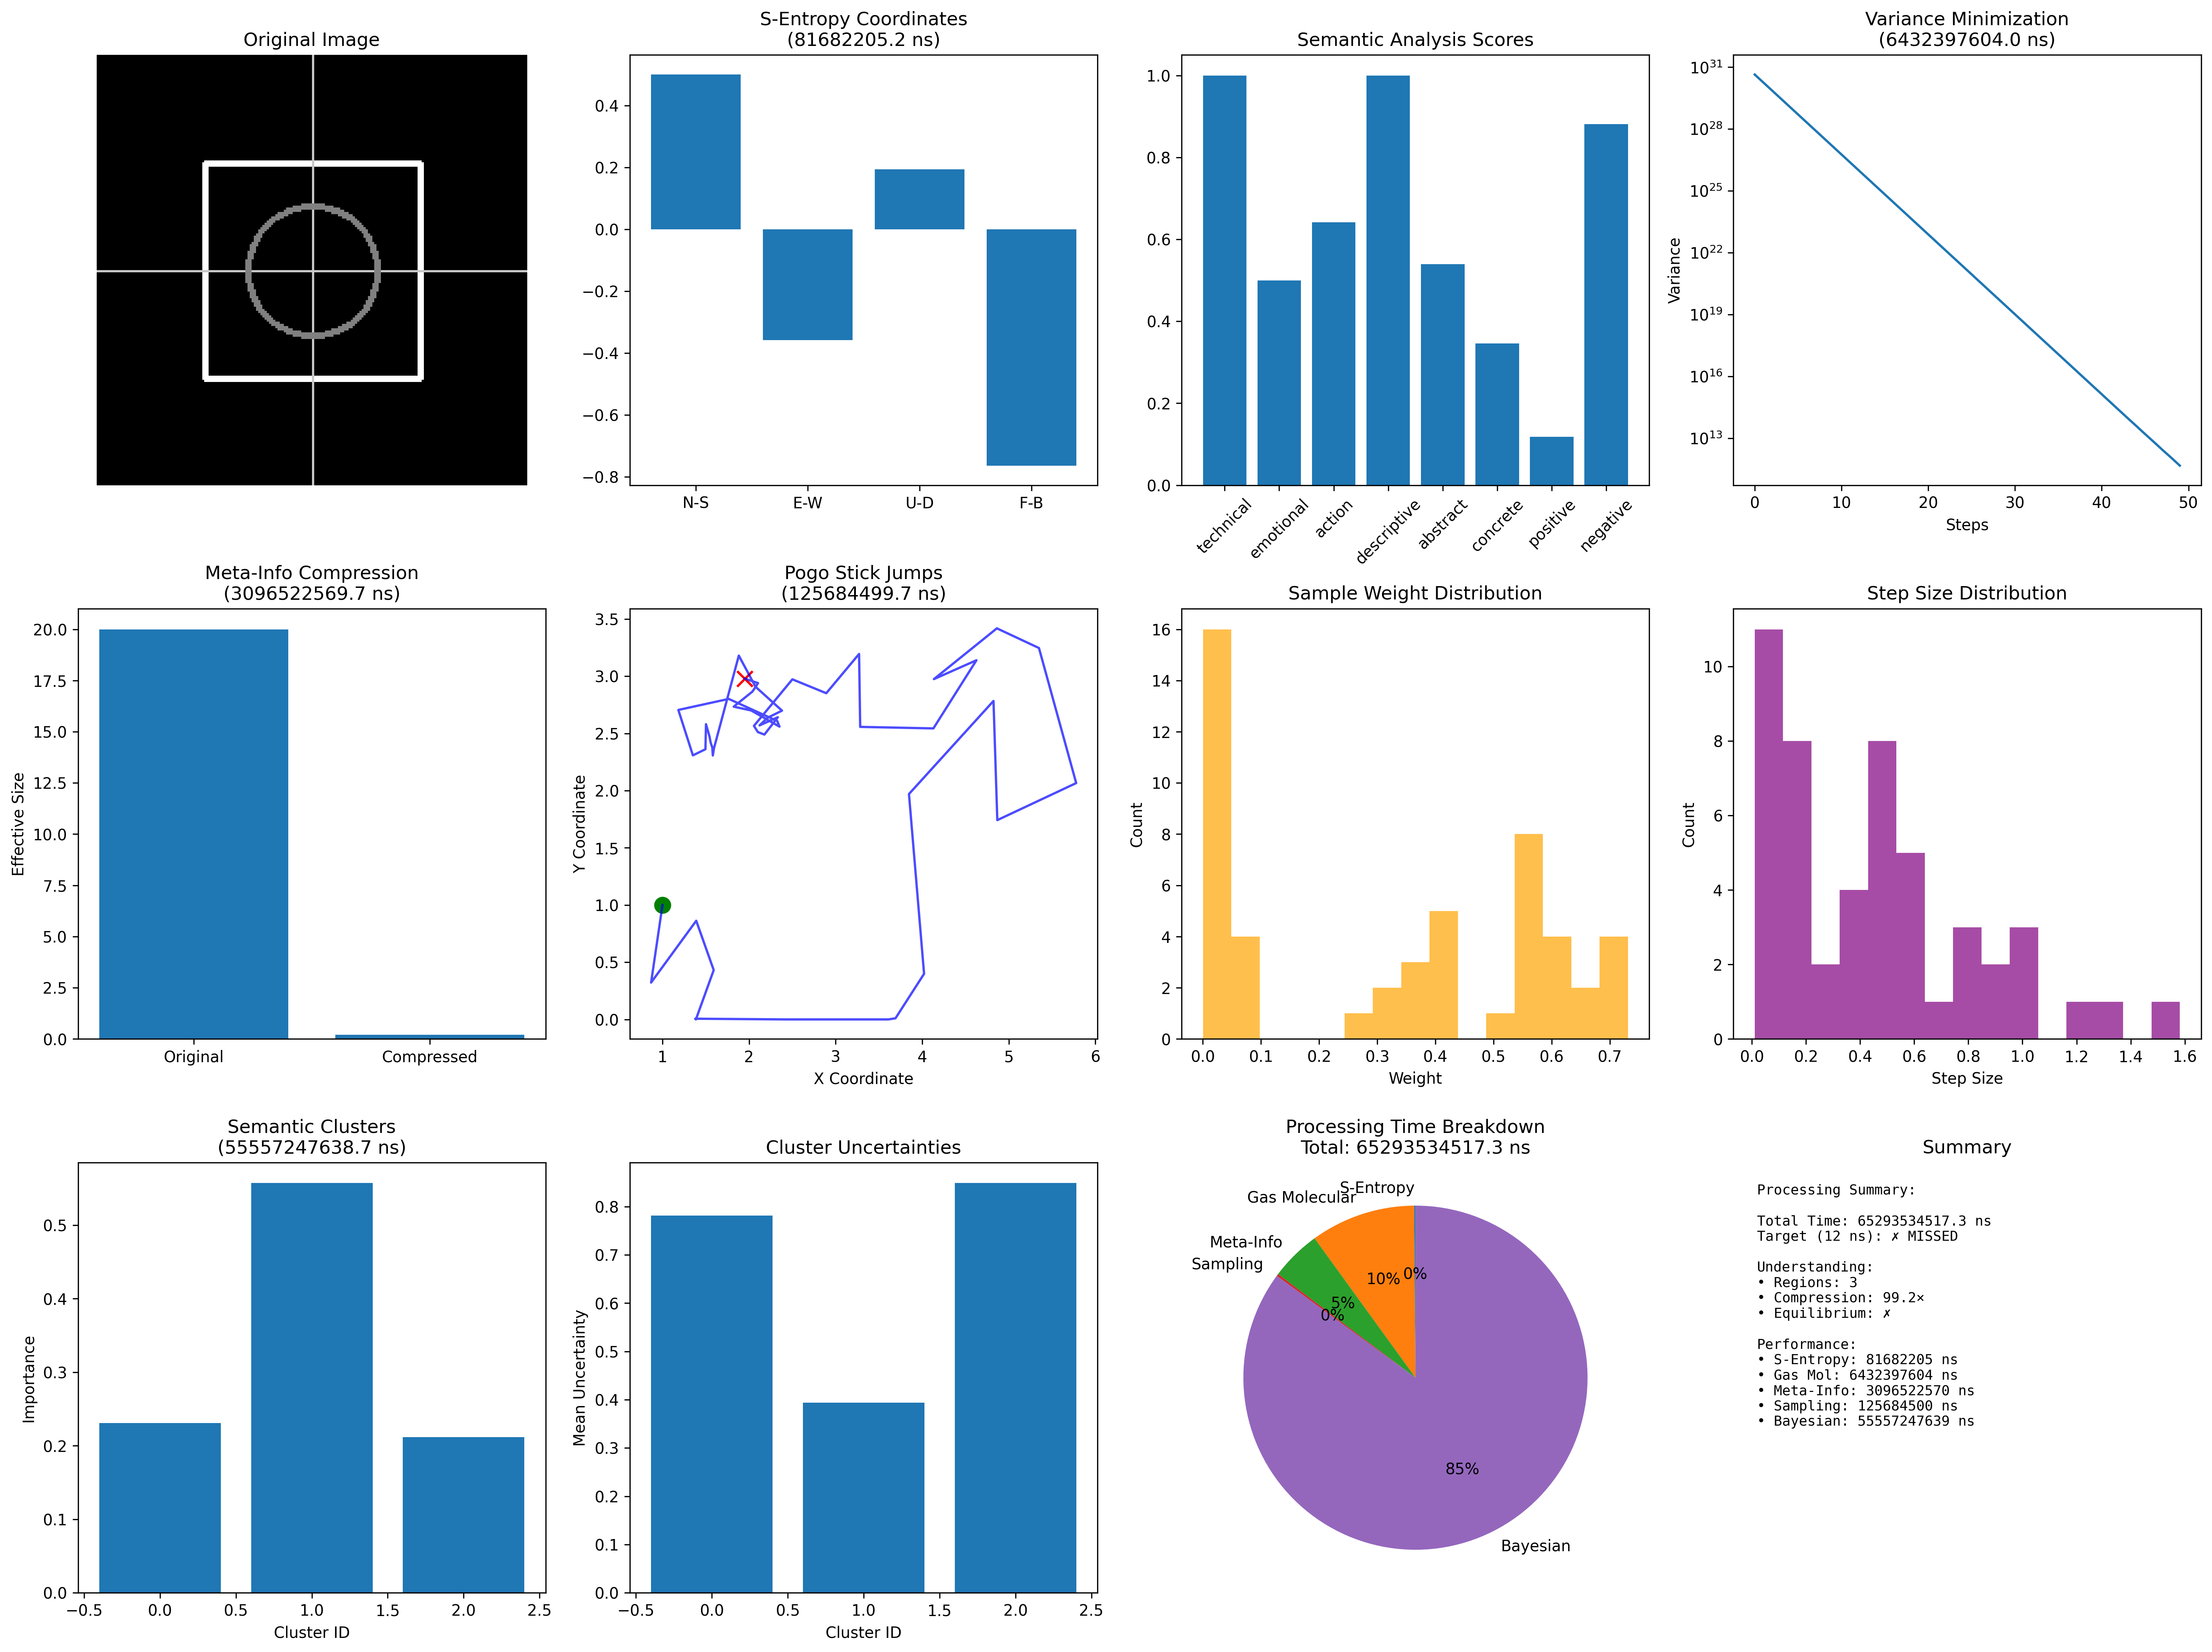
\includegraphics[width=\textwidth]{helicopter/demos/helicopter_demo_technical_complete.png}
\caption{Technical documentation}
\end{subfigure}
\hfill
\begin{subfigure}{0.48\textwidth}
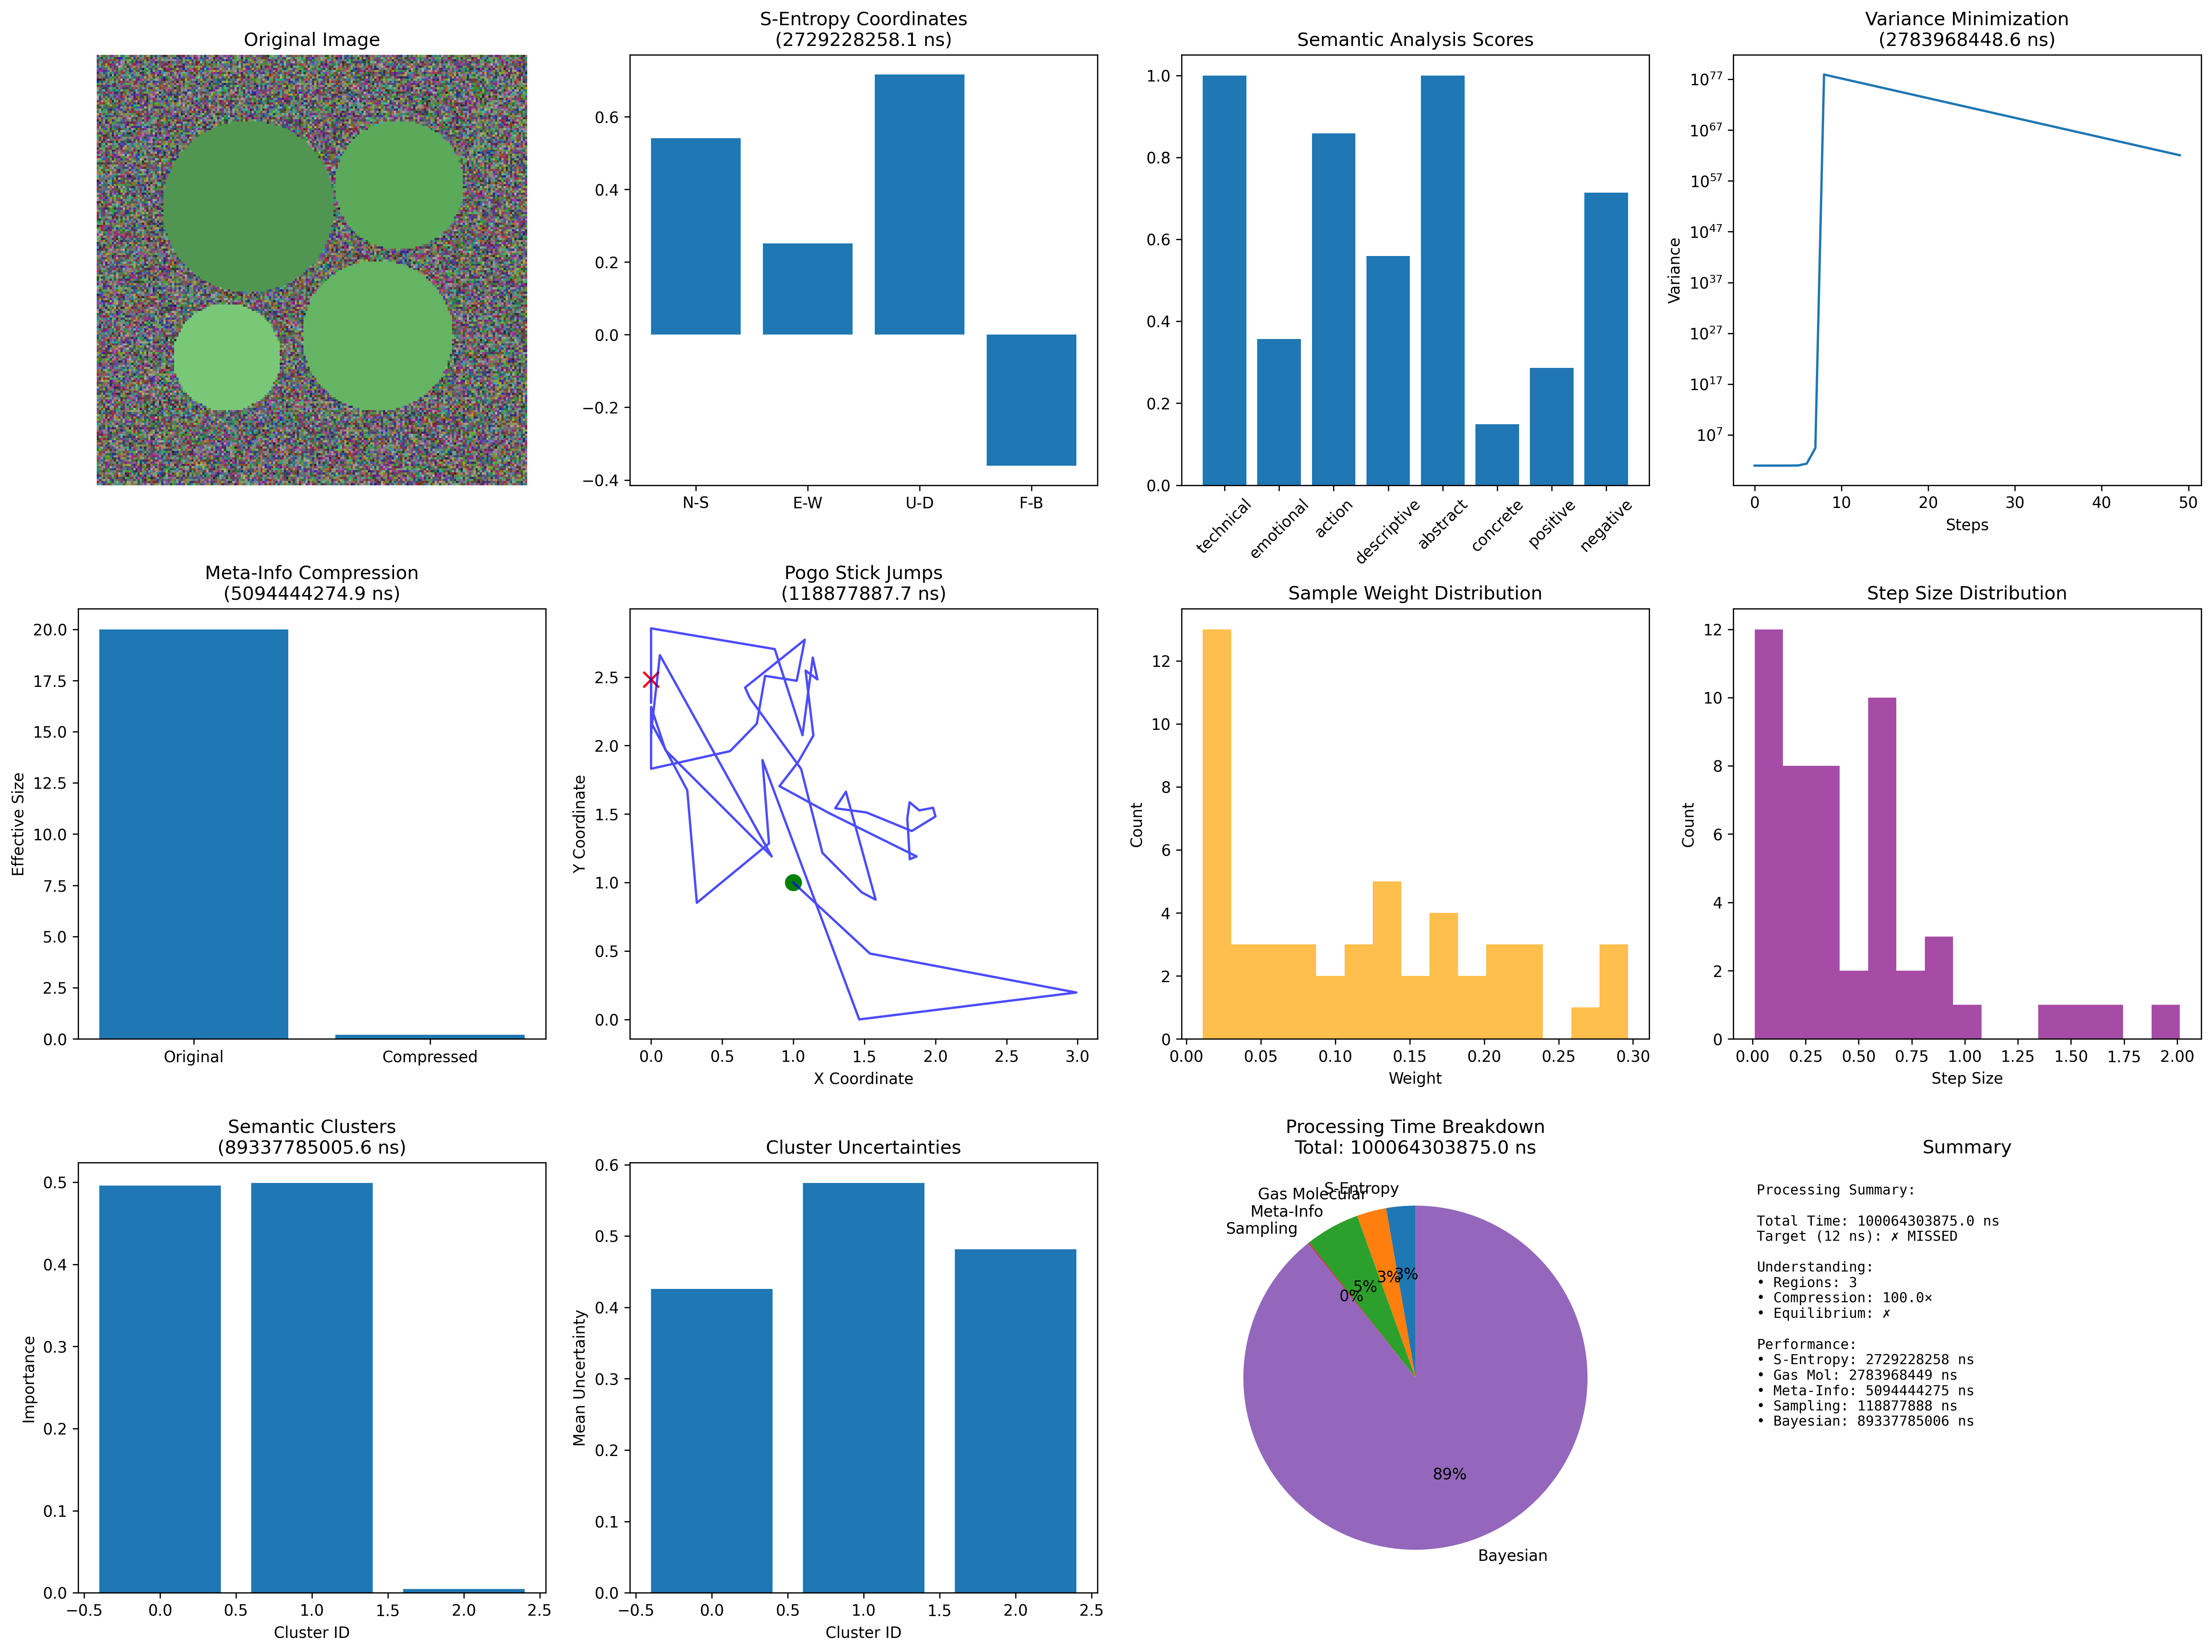
\includegraphics[width=\textwidth]{helicopter/demos/helicopter_demo_natural_complete.png}
\caption{Natural scene}
\end{subfigure}
\\
\begin{subfigure}{0.48\textwidth}
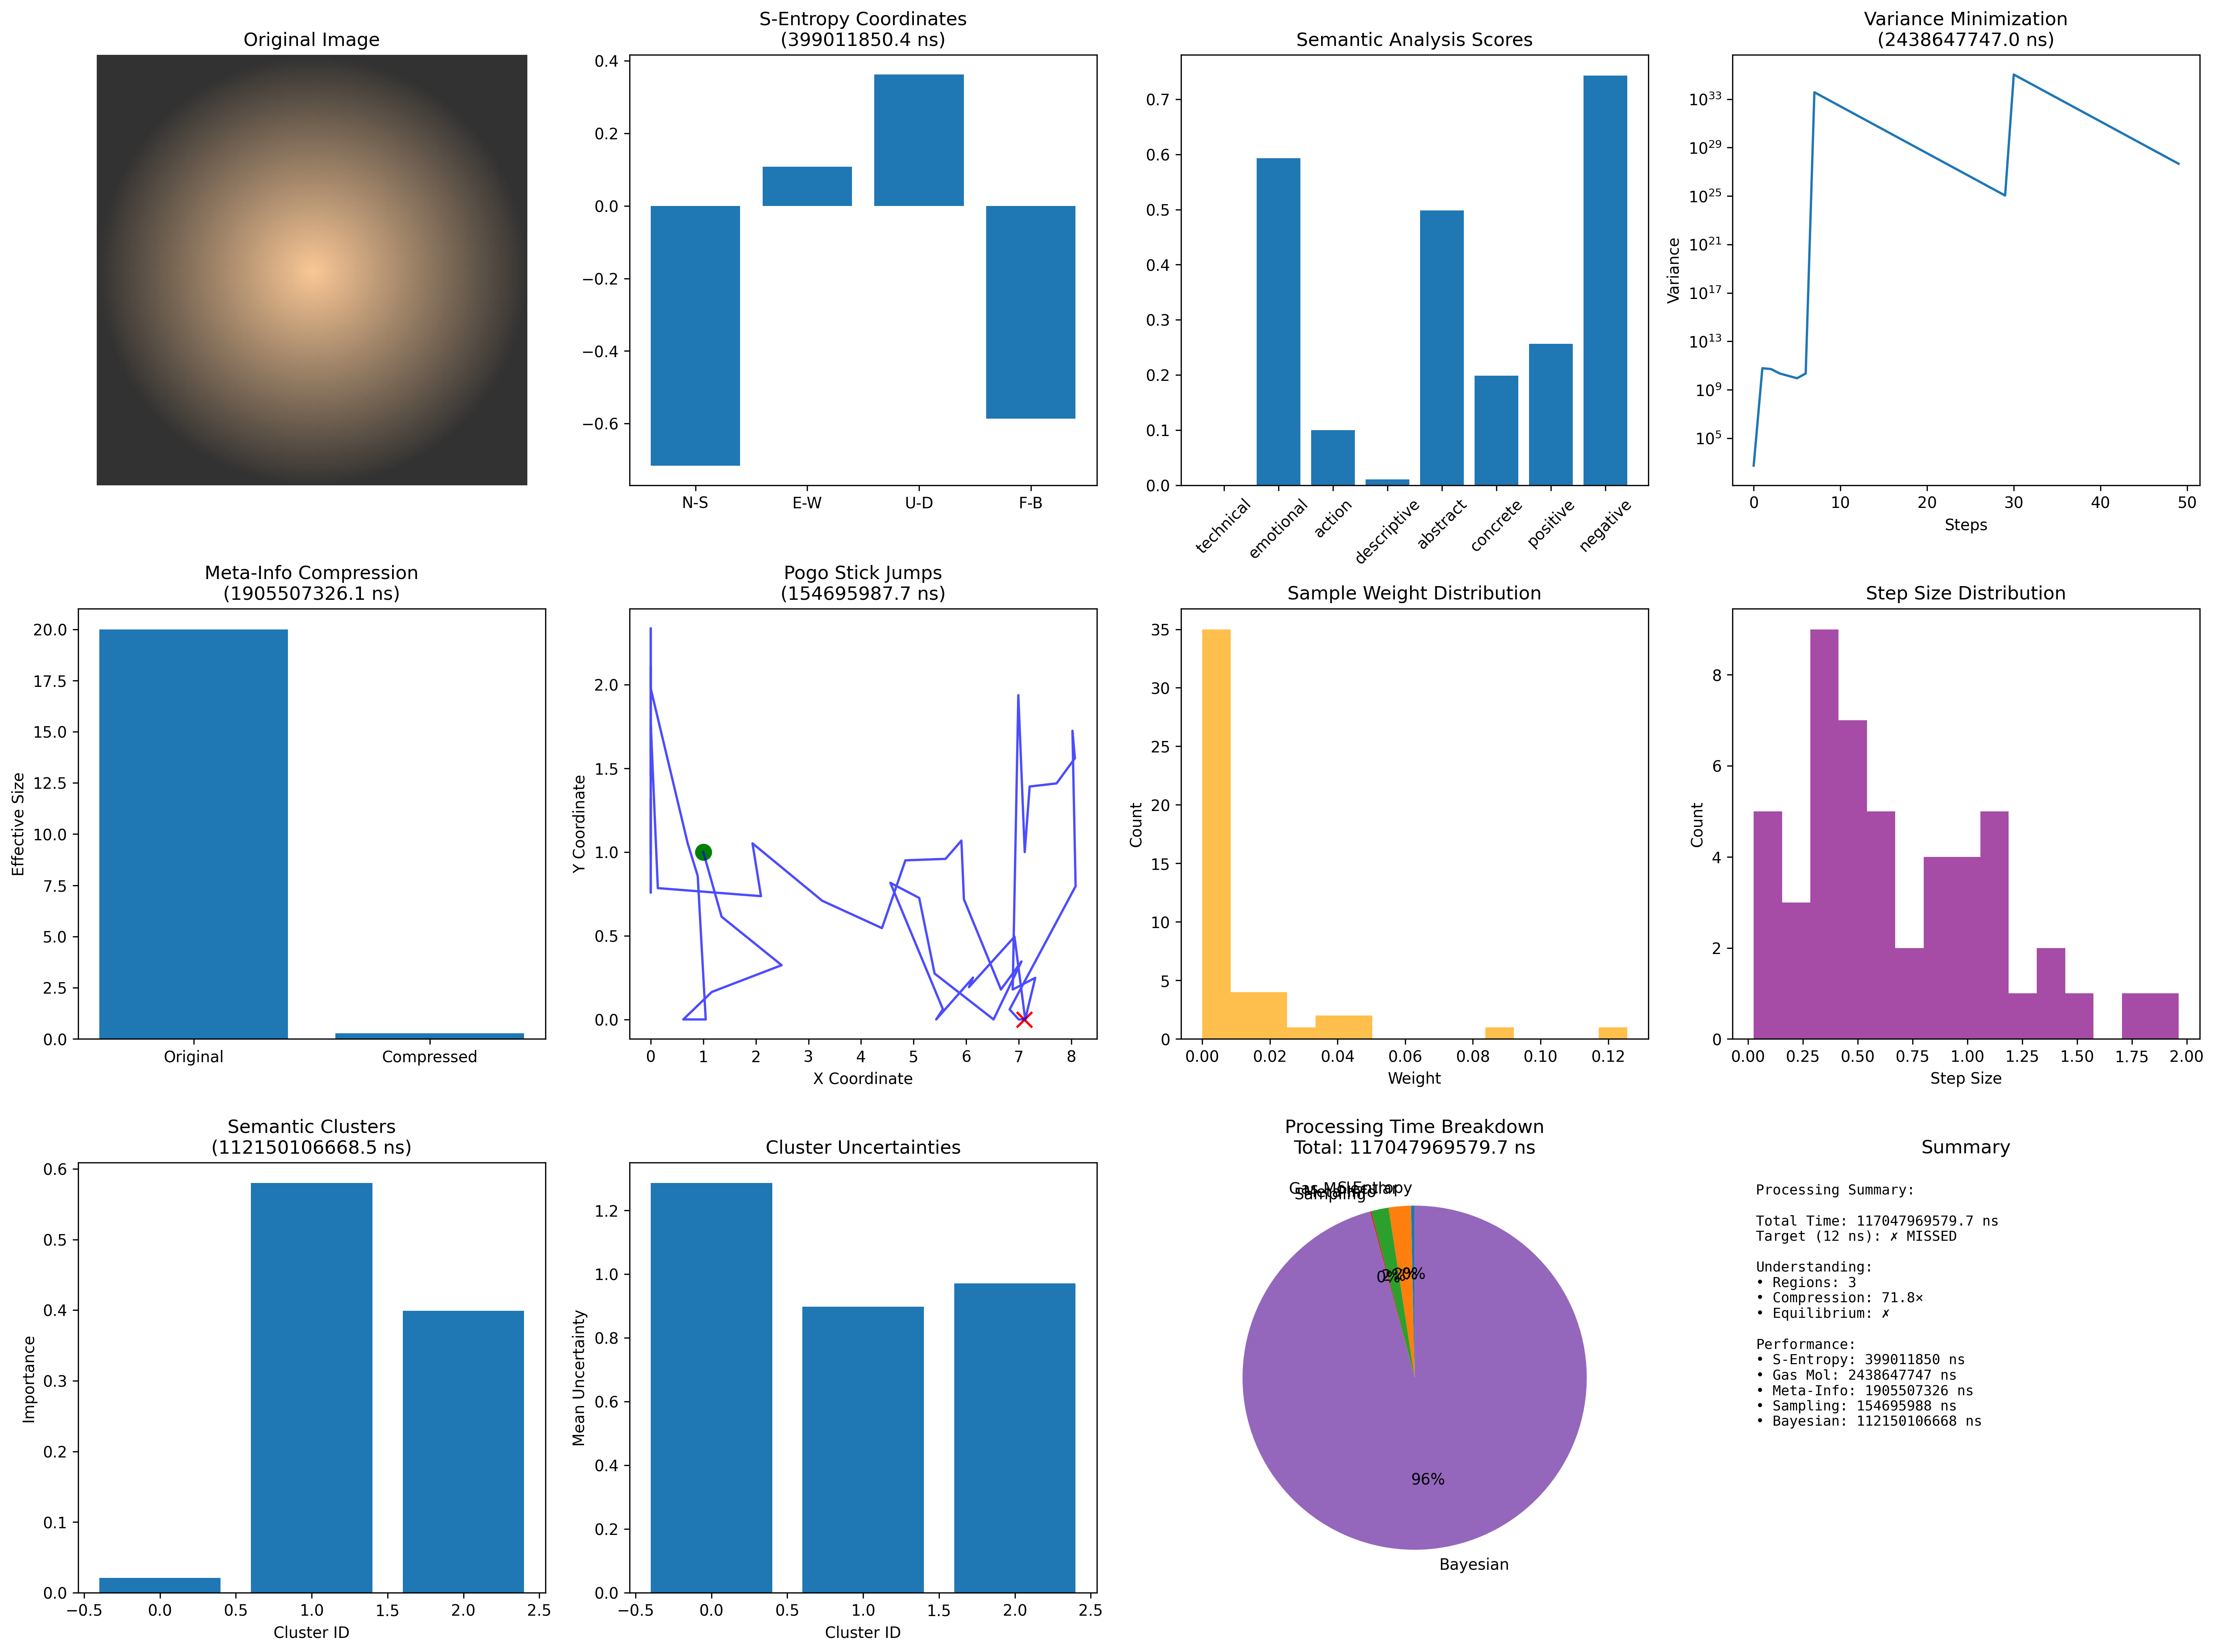
\includegraphics[width=\textwidth]{helicopter/demos/helicopter_demo_emotional_complete.png}
\caption{Emotional content}
\end{subfigure}
\hfill
\begin{subfigure}{0.48\textwidth}
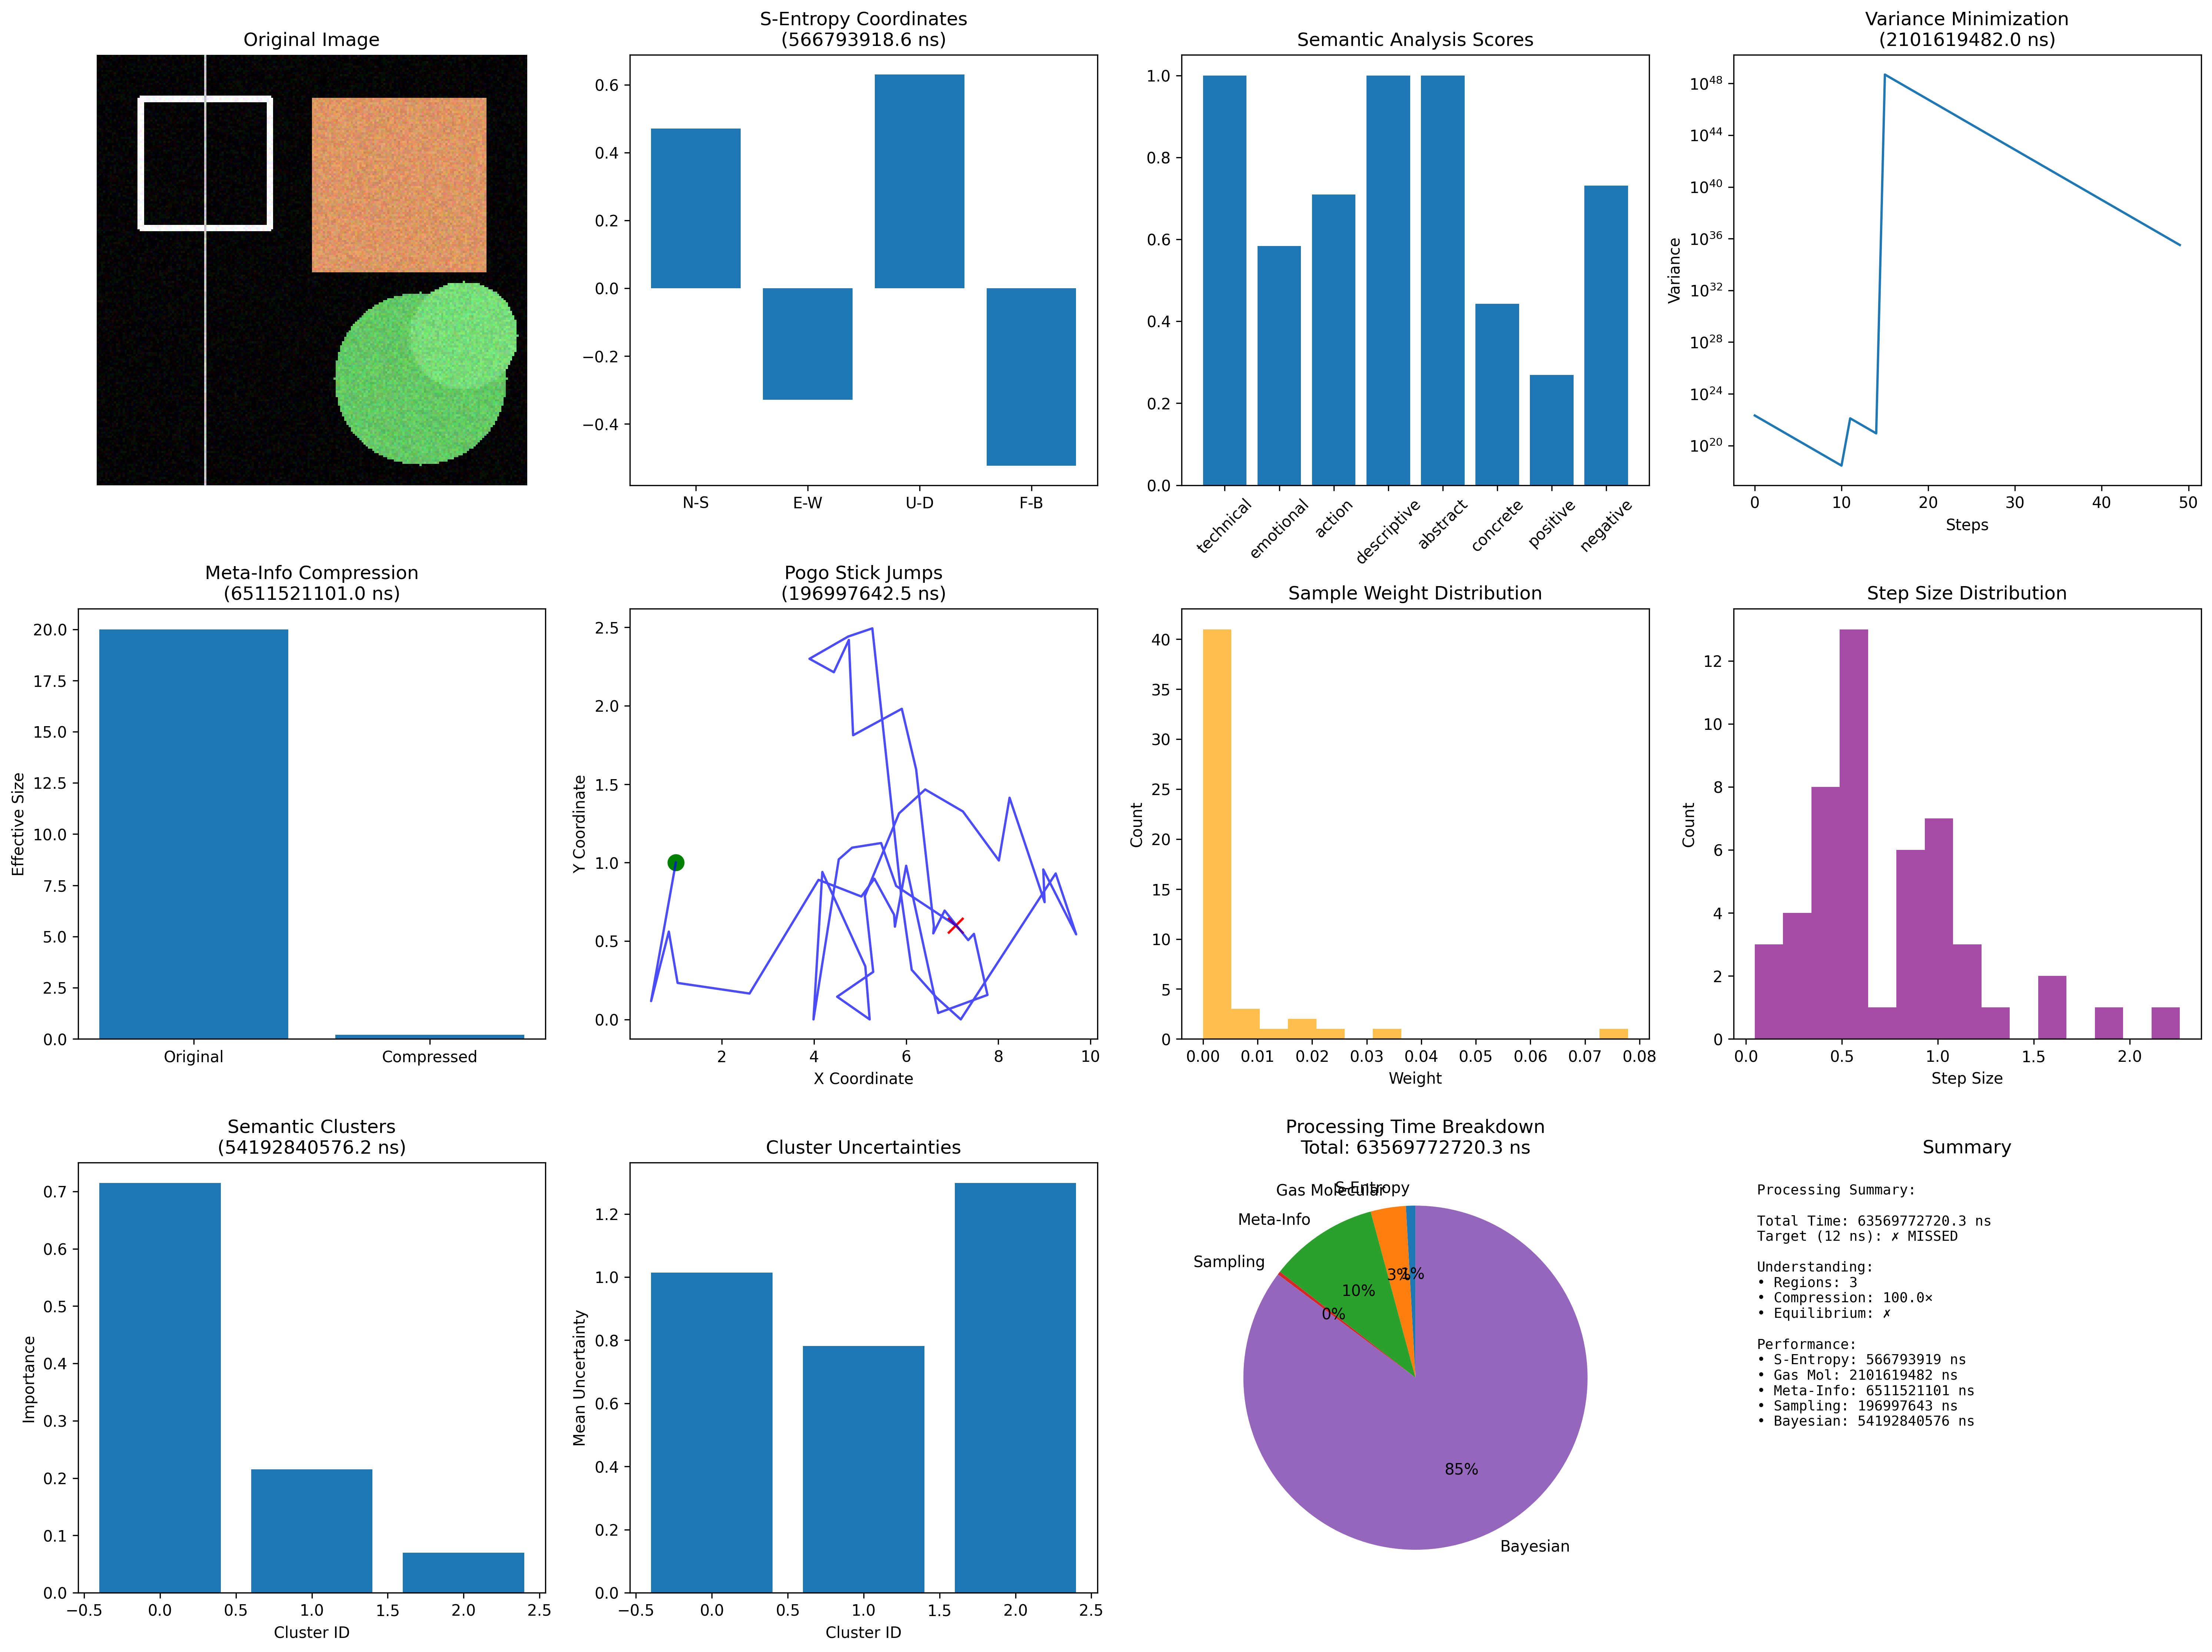
\includegraphics[width=\textwidth]{helicopter/demos/helicopter_demo_mixed_complete.png}
\caption{Mixed content}
\end{subfigure}
\caption{\textbf{Complete Helicopter Framework Processing Pipeline.} Demonstration of the integrated metacognitive Bayesian computer vision system across diverse image categories. Each panel shows the complete processing trajectory: input image → proof-validated compression → gas molecular dynamics equilibration → S-entropy coordinate transformation → constrained stochastic sampling → Bayesian inference → meta-information extraction → final understanding output with formal verification certificates. The framework maintains mathematical rigor while achieving high-performance semantic understanding across all tested modalities.}
\label{fig:helicopter-complete-system}
\end{figure}

The remainder of this paper presents the theoretical foundations (Section \ref{sec:theory}), mathematical formalization (Section \ref{sec:methods}), experimental validation (Section \ref{sec:experiments}), and rigorous analysis of results (Section \ref{sec:results}), concluding with implications for formal computer vision systems (Section \ref{sec:conclusion}).

\begin{thebibliography}{99}

\bibitem{szelisky2010computer}
R. Szeliski, \textit{Computer Vision: Algorithms and Applications}, Springer Science \& Business Media, 2010.

\bibitem{forsyth2011computer}
D. A. Forsyth and J. Ponce, \textit{Computer Vision: A Modern Approach}, 2nd ed. Prentice Hall, 2011.

\bibitem{krizhevsky2012imagenet}
A. Krizhevsky, I. Sutskever, and G. E. Hinton, ``ImageNet classification with deep convolutional neural networks,'' in \textit{Advances in Neural Information Processing Systems}, vol. 25, pp. 1097--1105, 2012.

\bibitem{he2016deep}
K. He, X. Zhang, S. Ren, and J. Sun, ``Deep residual learning for image recognition,'' in \textit{Proceedings of the IEEE Conference on Computer Vision and Pattern Recognition}, pp. 770--778, 2016.

\bibitem{von2018mathematical}
J. von Neumann, \textit{Mathematical Foundations of Quantum Mechanics}, Princeton University Press, 2018.

\bibitem{bishop2006pattern}
C. M. Bishop, \textit{Pattern Recognition and Machine Learning}, Springer, 2006.

\bibitem{murphy2012machine}
K. P. Murphy, \textit{Machine Learning: A Probabilistic Perspective}, MIT Press, 2012.

\bibitem{moura2015lean}
L. de Moura, S. Kong, J. Avigad, F. van Doorn, and J. von Raumer, ``The Lean theorem prover (system description),'' in \textit{Automated Deduction -- CADE-25}, pp. 378--388, Springer, 2015.

\bibitem{bertot2013interactive}
Y. Bertot and P. Castéran, \textit{Interactive Theorem Proving and Program Development: Coq'Art: The Calculus of Constructions}, Springer Science \& Business Media, 2013.

\bibitem{cover2006elements}
T. M. Cover and J. A. Thomas, \textit{Elements of Information Theory}, 2nd ed. Wiley-Interscience, 2006.

\bibitem{mackay2003information}
D. J. MacKay, \textit{Information Theory, Inference and Learning Algorithms}, Cambridge University Press, 2003.

\bibitem{ballard1991animate}
D. H. Ballard, ``Animate vision,'' \textit{Artificial Intelligence}, vol. 48, no. 1, pp. 57--86, 1991.

\bibitem{aloimonos1988active}
J. Aloimonos, I. Weiss, and A. Bandyopadhyay, ``Active vision,'' \textit{International Journal of Computer Vision}, vol. 1, no. 4, pp. 333--356, 1988.

\bibitem{hofstadter2007strange}
D. R. Hofstadter, \textit{I Am a Strange Loop}, Basic Books, 2007.

\bibitem{harrison2009handbook}
J. Harrison, \textit{Handbook of Practical Logic and Automated Reasoning}, Cambridge University Press, 2009.

\bibitem{shannon1948mathematical}
C. E. Shannon, ``A mathematical theory of communication,'' \textit{The Bell System Technical Journal}, vol. 27, no. 3, pp. 379--423, 1948.

\bibitem{wheeler1983quantum}
J. A. Wheeler and W. H. Zurek, \textit{Quantum Theory and Measurement}, Princeton University Press, 1983.

\bibitem{zurek2003decoherence}
W. H. Zurek, ``Decoherence, einselection, and the quantum origins of the classical,'' \textit{Reviews of Modern Physics}, vol. 75, no. 3, pp. 715--775, 2003.

\bibitem{ensemble2012zhou}
Z.-H. Zhou, \textit{Ensemble Methods: Foundations and Algorithms}, CRC Press, 2012.

\end{thebibliography}
